\documentclass[a4paper,twosided,notoc]{tufte-book}
\usepackage[utf8]{inputenc}
% For nicely typeset tabular material
\usepackage{booktabs}
% For images
\usepackage{graphicx}
 
\hypersetup{colorlinks}	

%metadata for book
\author{Naveen Thakur}
\title{Statistics in Action}
\date{January 2021}
\publisher{Version 0.1}

\begin{document}
\maketitle
\begin{fullwidth}
	\tableofcontents
\end{fullwidth}


\chapter{Statistical Inference}
A 'sample statistic' such as the mean, variance or proportion is calculated using data obtained from an actual sample \sidenote{What is the mean of 0.12, 1.1, 0.9, 0.17, 0.08? These are the masses relative to the sun of the five nearest star-like objects in space. The summary data (statistic) is the requested mean and the list of solar masses the sample data.}
We're going to discuss how these statistics can be generalised to infer something about the population from which it came. Why is this important? Here's an example.

In 2014, American and European surveys showed that between $15\%-30\%$ of adult workers are involved in shift work \sidenote{\href{https://www.sciencedirect.com/science/article/abs/pii/S0369811414001230}{Impact of shift work on sleep and circadian rhythms}}. The survey paper looked specifically at the potentially dangerous effects of shift work on worker performance. However, by 2020 research \sidenote{\href{https://www.nature.com/articles/s41597-020-00709-6}{Brain activity and transcriptional profiling in mice under chronic jet lag}}is suggesting that shift work may be associated with far more types of 'adverse health outcomes' including increased risk of cardiovascular disorders, neurological diseases, cognitive defects and increased risk of mental illnesses.

Of course, the question is 'why'? Why is shift work affecting the brain/body and increasing the risk of various conditions? The title of the second paper mentioned above includes the intriguing phrase '...mice under chronic jet lag (CJL)'. It turns out that you can simulate shift work by inducing CJL in mice, by disrupting their exposure to light and dark. PET scans can then be used to examine the volume of activity within their brains (measured by glucose usage) and RNA sequencing used to show any disruption in gene expression that may be causing glucose changes. The results are startling in that after 34 days there are 'prominent and pervasive' changes in brain activity and that even after 10 days circadian gene expression \sidenote{\href{https://www.ncbi.nlm.nih.gov/pmc/articles/PMC3762864/}{Beautiful definition of circadian rhythms which affect body and brain:} "As the sun sets, nocturnal rodents begin to forage, nocturnal birds of prey begin their hunt while diurnal birds of prey sleep, filamentous fungi begin their daily production of spores, and cyanobacteria begin nitrogen fixation in an environment of low O2 after the day’s photosynthesis. As the sun rises the next morning many plants have positioned their leaves to catch the first rays of light and many humans sit motionless in cars on a nearby gridlocked highway...the obedience to temporal niches in all organisms is governed by a molecular circadian clock...not driven by sunlight, but synchronized by the 24 hour patterns of light and temperature produced by the earth’s rotation."} undergoes substantial change. 

But our question is very specific: only 15 mice were used to test the effect of CJL. But there are reportedly 10s of millions \sidenote{That's a  \href{https://www.sciencemag.org/news/2021/01/how-many-mice-and-rats-are-used-us-labs-controversial-study-says-more-100-million}{gory and statistically controversial number} in an area of ethical minefields. 6 mice were sacrificed in this study - what's your evaluation?} of mice in laboratories being used for research as you read this. Surely we should test all those mice to be sure?! It's obvious why each mouse in the world was not subject to CJL, PET, brain dissection and RNA sequencing. The time and cost would be prohibitive and a world without mice unthinkable. So why are we entitled to generalize and to what degree?


\chapter{Central Limit Theorem - how to catch a cheat}
\section{Sampling Distribution}
Generalising a conclusion from particular sample to its wider population is called statistical inference. But how is that jump made? What is hidden within a single sample that might help us infer something about its wider population? In fact, the answer lies within the study of \textbf{many} samples. Imagine drawing a random sample of fixed size from the population. It is a 'random sample' because each member of the population has an equal chance of being selected. Now record the mean \sidenote{From now on we focus on the well known sample statistic 'the mean'. This will reveal one of the mighty pillars of statistical inference.} of that sample and repeat the process of 'drawing a sample and recording the mean' a large number of times. Statisticians can't resist the urge to group these means into a theoretical construct known as the sampling distribution. It is a distribution because each of these means will differ to some degree as each sample is more or less different from the other.

As an aside, do not confuse 'sampling distribution' with a 'sample distribution': the 'sampling' describes the shape of the mean when sampling repeatedly, while the 'sample' concerns the shape of the data within a single sample.

And it is within the sampling distributions that statisticians have discovered amazing regularities which act like a bridge from the particular to the general upon which inference can pass. These regularities are captured by the 'central limit theorem'.

The central limit theorem says that if you take a large number of samples of fixed size then the distribution of those sample's means will approach a normal distribution. Further, those sample means will cluster around the mean value of the wider population. Finally, the spread of the sample means (standard deviation) will approach the population's standard deviation divided by the square root of the fixed sample size.

The theorem has been shown to be true in a wide range of circumstances and is a central engine of statistical inference. It is these regularities that connect characteristics of individual samples to population parameters.

\subsection{Catching cheats}
This regularity described by the central limit theorem can be used to detect dodgy research articles - if an RCT is performed and the data doesn't match the CLT (often over years) then something is afoot.

Here's a rather innocent title published in 2012 'The analysis of 168 randomised controlled trials to test data integrity'. 

RCT should distribute height randomly across control and treatment groups. Crass diagram showing non-random vs random distribution?

\subsection{Sample Error and Standard Error}

Earlier we explained why the mean differed between random samples. The 'sample error' or 'sample variation' (statisticians often uses the term 'error' to indicate 'noise' or 'variation' and not 'error' as in mistake) describes the degree to which a particular sample mean deviates from the population mean. Given the CLT, we expect these sample errors to vary in magnitude and resemble a normal distribution. The standard deviation of these errors is renamed 'standard error'. Therefore, the standard error gives an indication of how spread out are the magnitudes of the sample errors.

\subsection{CLT in action}
Quite often in the previous discussion we have spoken about the population parameter as though it's known which begs the question 'If you already know the population parameter - there isn't much left to infer?!'. 

Of course, we often don't know the population mean. But we can hypothesize its value and test a sample mean to see whether that value is so unusual that the hypothesized population mean looks ludicrous. We can do this because given a hypothesized mean, the CLT tells us that a distribution of the sample mean approximates a normal distribution. And it is this distribution that allows us to work out exactly how (un)likely we were to get the actual sample in our hands if the hypothesized mean were true. 

\subsection{The example}
The gallbladder is a small pouch nestled under the liver where it collects a fluid known as bile used to break down fats during digestion. Unlike many other organs, it's not essential to survival and can be safely removed if it develops any problems. This surgical procedure is known as a cholecystectomy ('coal-eh-sis-tec-tuhmy'). Modern surgery has made a cholecystectomy into a keyhole procedure in which case it is called a 'laparoscopic cholecystectomy'. However, the operation is usually performed under general anaesthesia which in and of itself can result in post-operative nausea and vomiting (PONV). This can be a problem as preventing a would from healing, dehydration and increased pain \sidenote{\href{https://handbook.ggcmedicines.org.uk/guidelines/pain-post-operative-nausea-and-vomiting-and-palliative-care-symptoms/management-of-postoperative-nausea-and-vomiting-ponv/}{Details here}}.

In 2004, Japanese anaesthetist Dr Yoshitaka Fujii and colleagues decided to test an anaesthetic drug called Granisetron, used to prevent nausea after chemotherapy. 

The key point for now is that they used 'Random Controlled Trials' (RCT). The theory is simple. Pick people at random and assign them to 5 groups. One group is the control group (no treatment) while each of the other groups receives a different dose of Granisetron. This maximizes the chance that any effects detected are due to the drug and not to any other variable. For example, if the women were split into two groups (say over 50 and under 50), and the women over 50 responded strongly to treatment, then what caused the improvement?. Perhaps women over 50 would have minimal PONV without the drug. By randomizing we ensure each group has a healthy mix of participants and any effect is morel likely to be due to treatment. Now we will have women under 50 and over 50 responding well to treatment. This is a super important basis for clinical trials.

They concluded that over $20\mu g/kg^{-1}$ but less than $80\mu g/kg^{-1}$ of Granisetron made a dramatic improvement to the rate of those suffering PONV after laparoscopic cholecystectomy.

Let's examine some of the simpler results - something is lurking!

In the results table/ below, each measured value is written in the form 'mean (standard deviation)'. The first column is a description of each variable measured for each of the 100 participants. The second column gives the value of those variables for the 20 participants in the placebo group (control group). The other four groups, each containing 20 participants, were randomly assigned to take differing doses of Granisteron (micro grammes per kilogram of body weight). The last column is the mean of the means and standard deviations in the previous five columns (CLT).

\begin{table}[h]
	\begin{center}
		\footnotesize
		\begin{tabular}{lcccccc}
			\toprule
			\multicolumn{1}{l}{Variable} & \multicolumn{1}{c}{Placebo} & \multicolumn{4}{|c|}{Granisteron $\mu g/kg^{-1}$} & \multicolumn{1}{r}{$\approx\mu_{pop}$} \\
			 &  & 10 & 20 & 40 & 80 & \\
			\midrule
			Age (y)                         & 46 (8)   & 47 (7)   & 45 (11)  & 47 (10)  & 50 (11)  & 47 (9.4)   \\
			Height (cm)                     & 159 (10) & 158 (9)  & 155 (11) & 157 (10) & 159 (9)  & 158 (9.8) \\
			Weight (kg)                     & 57 (7)   & 57 (9)   & 54 (7)   & 54 (8)   & 58 (8)   & 56 (8.2)   \\
			Surgery (min)                   & 86 (35)  & 92 (31)  & 83 (34)  & 87 (36)  & 92 (27)  & 88 (32.6)  \\
			Anaesthetic (min)               & 106 (35) & 117 (33) & 106 (36) & 112 (37) & 118 (29) & 112 (34) \\
			Fentanyl\footnotemark{} ($\mu$g) 				& 103 (79) & 98 (73)  & 93 (73)  & 98 (79)  & 105 (86) & 99 (78)  \\
			LMP\footnotemark{} (d)       & 16 (3)   & 16 (3)   & 16 (3)   & 16 (3)   & 16 (3)   & 16 (3) \\
			\bottomrule
		\end{tabular}
	\end{center}
	\caption{Granisetron dosage for five groups}
	\label{tab:heading-styles}
\end{table}
\footnotetext{Last Menstrual Period}
\footnotetext{Fixed dosage at start, with additional amounts during operation (recorded). It is a pain killer over 100 times more powerful than morphine! Read the story in the startlingly named  \href{https://www.jpain.org/article/S1526-5900(14)00905-5/pdf}{'The Journal of Pain'}. Yikes!}

Examine each row from left to right, and see if you notice anything odd. Given a random assignment of women to each group, the last row is surprisingly uniform. Let's park that for now and let's look at the rest of the data.

Thanks to the CLT, whether each sample measures age or weight is irrelevant. The differences between the population mean and each sample mean can be approximated by same structure - that of a normal distribution. But what of the mean and deviation of this curve? Using the well known sample 'z-score' we can transform each of the 35 results into a standardised score. These scores will have a mean and variance of their own that will allow us to examine their shape.

Let's look at the first row. We take the population mean and standard deviation to be $\mu=47$ and $\sigma=9.4$. The equation for a XXXX is $\frac{\overline{\mu} - \mu}{\sigma/\sqrt{n}}$. Then for the first row $SEM=9.4/\sqrt{20} = 2.10$. Now let's look at the Placebo column. We calculate its score as $\frac{46 - 47}/2.10 = -0.48$ to two decimal places. The rest of the rows are calculated accordingly.

\begin{table}[h]
	\begin{center}
		\footnotesize
		\begin{tabular}{lcccccc}
			\toprule
			\multicolumn{1}{l}{Variable} & \multicolumn{1}{c}{SEM} & \multicolumn{1}{c}{Placebo} & \multicolumn{4}{|c|}{Granisteron $\mu g/kg^{-1}$} \\
			&  & 10 & 20 & 40 & 80 & \\
			\midrule
			Age (y)                         & 2.10  & -0.48 & 0.00  & -0.95 & 0.00  & 1.43 \\
			Height (cm)                     & 2.19  & 0.64  & 0.18  & -1.19 & -0.27 & 0.64 \\
			Weight (kg)                     & 1.74  & 0.57  & 0.57  & -1.15 & -1.15 & 1.15 \\
			Surgery (min)                   & 7.29  & -0.27 & 0.55  & -0.69 & -0.14 & 0.55 \\
			Anaesthetic (min)               & 7.60  & -0.76 & 0.68  & -0.76 & 0.03  & 0.82 \\
			Fentanyl ($\mu$g) 				& 17.44 & 0.21  & -0.08 & -0.37 & -0.08 & 0.32 \\
			LMP (d)       & 0.67  & 0.00  & 0.00  & 0.00  & 0.00  & 0.00 \\
			\bottomrule
		\end{tabular}
	\end{center}
	\caption{Granisetron dosage for five groups}
	\label{tab:heading-styles}
\end{table}

As a result, each of the 35 differences in mean can be mapped to the same distribution. What are its parameters? The mean of all 35 values is approximately zero but the standard deviation is $0.6393103$. Let's compare that to the ideal standard normal distribution to be expected from truly random values.

\begin{figure}
	\centering
	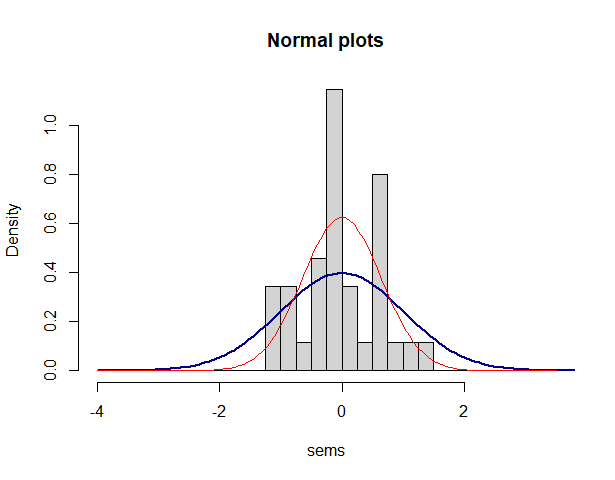
\includegraphics[width=0.7\linewidth]{screenshot001}
	\caption{}
	\label{fig:screenshot001}
\end{figure}
The blue curve is a standard normal distribution but the red curve is the plot derived from the samples above. The histogram shows the results in $0.25$ standard deviation increments. The analysis shows something interesting. There red curve has squeezed together because, as the histogram indicates, the results have cut off abruptly at the edges. If the RCT were random, you would expect more results around the edges which would tend to spread the red curve toward the black one.



\end{document}
